\setcounter{page}{1}
\clubpenalty=10000 
\widowpenalty=10000
%%%%%%%%%%%%%%%%%%%%%%%%%%%%%%%%%%%%%%%%
%      Шапка экспертной организации  
%%%%%%%%%%%%%%%%%%%%%%%%%%%%%%%%%%%%%%%%
%
%%%%%%%%%%%%%%%%%%%%%%%%%%%%%%%%%%%%%%%%%
%
%   Экспертная организация ИП
%
%%%%%%%%%%%%%%%%%%%%%%%%%%%%%%%%%%%%%%%%%
\noindent
\begin{pspicture}(21mm,21mm)
\obeylines
\psbarcode{%
	%\NomerDoc от \окончено
	BEGIN:VCARD^^J
	VERSION:4.0^^J
	N:Мраморнов; Александр; Вчеславович^^J
	FN:Александр Мраморнов^^J
%	ORG:IP Alexandr Mramornov^^J
	TITLE: эксперт
	ORG: ИП
	URL:http://www.yourexp.ru^^J
	EMAIL:yourexpert.mramornov@gmail.com^^J
	TEL:+7-918-451-6611^^J
%	ADR:г. Краснодар, с/т № 2 А/О «Югтекс», ул. Зеленая, 472^^J
	END:VCARD
}{width=1.0 height=1.0}{qrcode}%
\end{pspicture}

 %%% Добавлен QR-Code
\vspace{-4mm}
\begin{center}
	\large\textbf{ИНДИВИДУАЛЬНЫЙ\quad ПРЕДПРИНИМАТЕЛЬ  \\[-1.5mm] МРАМОРНОВ  АЛЕКСАНДР ВЯЧЕСЛАВОВИЧ \\[-5.5mm]}
	%  
	\noindent\rule{\textwidth}{2pt}\\[-6mm]  % Горизонтальная линия
	% \line(1,0){460}% (1,0) -горизонтальная линия, и (0,1) - вертикальная 
\end{center}

\begin{center}
	\begin{footnotesize}
		%	\small\textbf\setlength   	%\raisebox{5mm}
		\vspace{-2.5mm}г. Краснодар, с/т № 2 А/О «Югтекс», ул. Зеленая, 472, 
		Телефон: 8-918-451-66-11, e-mail: 4516611@gmail.com\\ [-2mm]{ИНН\quad 231200665168\quad ОГРНИП \quad 310231220400043}
	\end{footnotesize}	\\[10mm]
\end{center}


\begin{flushright}
% 
	 \hfill	Краснодар, 2023    \\[8mm]
\end{flushright}  
\begin{center}
	\LARGE\textbf{АКТ ЭКСПЕРТНОГО ИССЛЕДОВАНИЯ}
	\bigskip\\[-5mm] 
	\textbf{  {\normalsize № \NomerDoc\,  от \dataend}}
\end{center}
\par
\vspace{4mm}

%\noindent на <<заключение эксперта № 00182/18 по гражданскому делу № 2-802/19 по иску \иск>>\\


%%%%%%%%%%%%  Если независимая
\vspace{2mm}
\noindent %\dog\, владелец транспортного средства \тс\, регистрационный знак \грз \,  \владелец, \, проживающий: \адресвладельца \, обратился с заявление об определении износа принадлежащего ему транспортного средства на момент дорожно-транспортного происшествия, имевшего место \датадтп. %  составлен на основании	обращения владельца транспортного средства 40ОС277336%договора № \NomerDoc\,  \dog \,  возмездного оказания услуг.
Составлен на основании	договора № \NomerDoc\,от \датадоговора\, возмездного оказания услуг   по проведению независимой технической экспертизы (далее экспертиза)  транспортного средства \тс\, регистрационный знак \грз\, и письменного заявления заказчика \заказчик, \адресзаказчика\,  о проведении экспертизы.

\paragraph*{}
%Исследование произвели  специалисты:
Исследование произвёл  специалист
%{\small ООО "ЮЖНО-РЕГИОНАЛЬНАЯ ЭКСПЕРТНАЯ ГРУППА"}
\,  Мраморнов Александр Вячеславович, имеющий высшее  образование по специальности «техническая физика», диплом РВ №311964 от 28.02.1989, квалификация -- инженер-физик, специальное образование в области независимой технической экспертизы транспортных средств: Диплом ПП-I № 424167, квалификация: эксперт-техник (специализация 150210 специальности 190601.65 – Автомобили и автомобильное хозяйство), состоящий в Государственном реестре экспертов-техников (№ в реестре 256, https://data.gov.ru/opendata/7707211418-experts, специальное образование в области оценки: Диплом ПП-1 № 037211 Российской экономической академии им. Г.В. Плеханова, квалификация -- оценка и экспертиза объектов и прав собственности,   общий трудовой  стаж 30 лет, стаж  экспертной работы  12 лет. 

%%%%%%%% ВВС
%Вовчук Валерий Сергеевич, эксперт-автотехник,  имеющий высшее техническое образование, квалификацию «Инженер по эксплуатации автомобильной техники»,  квалификацию государственного судебного эксперта по специальностям: 2.1«Исследование обстоятельств дорожно-транспортного происшествия», 2.2«Исследование технического состояния узлов и деталей транспортного средства», 2.3«Исследование следов столкновения на транспортных средствах и месте дорожно-транспортного происшествия» (транспортно-трасологическая диагностика), 2.4«Исследование маркировочных обозначений транспортных средств», стаж экспертной работы 23 года (из них 15 лет государственный эксперт МВД РФ).

\par Заключение подготовлено по месту фактического расположения ИП по адресу: г. Краснодар, с/т № 2 А/О «Югтекс», ул. Зеленая, 472.
\vspace{4mm}  % Шапка организации ООО ЮРЕКСГРУП
%
%%   вопросы экспертизы
\subsection{Вопросы экспертизы}
%Заказчик поручает, а Исполнитель принимает на себя обязательство выполнить Заказчику  комплекс работ в виде автотехнических исследований автомобиля Mazda 6, VIN RUMGJ52\-6802007133 (дата начала гарантии 07.05.2018 г.), по следующим вопросам:
\begin{enumerate}
	\item  <<Связано ли повреждение панели рамки радиатора слева и брызговика с лонжероном переднего левого автомобиля ВАЗ 21099 с указанным ДТП?>>	
\end{enumerate}

\addcontentsline{toc}{section}{Использованные нормативы и источники информации}
%
%\left( \addcontentsline{toc}{section}{Использованные нормативы и источники информации}

\subsection{Использованные нормативы и источники информации}
%
\begin{enumerate}
\item 
Махнин\,Е.\,Л., Новоселецкий\, И.\,Н., Федотов\, С.\,В. \emph{Методические рекомендации по проведению судебных автотехнических экспертиз и исследований колёсных транспортных средств в целях определения размера ущерба, стоимости восстановительного ремонта и оценки} // -- М.: ФБУ РФЦСЭ при Минюсте России, 2018.-326 с.  ISBN 978-5-91133-185-6.
%
\item ТУ 017207-255-00232934-2014 \emph{Кузова автомобилей LADA. Технические требования при приёмке в ремонт, ремонте и выпуске из ремонта предприятиями дилерской сети ОАО "АВТОВАЗ"}//  ОАО НВП "ИТЦ АВТО", 2014
%
\item Смирнов  В.Л., Прохоров  Ю.С., Боюр В.С.  и др. \emph{Автомобили ВАЗ. Кузова. Технология ремонта, окраски и  антикоррозионной защиты. Часть II}// - Н.Новгород: АТИС, 2001.- 241с.
%
\item 
Савич Е.Л. \emph{Техническое  обслуживание  и  ремонт  легковых  автомобилей} : учеб. пособие / Е.Л. Савич, М.М. Болбас, В.К. Ярошевич ; под общ. ред. Е.Л. Савича. -Мн. : Вышэйшая школа,  2001. - 479 с. - ISBN985-06-0502-2.
%
\item 
Автомобили ВАЗ-2121, 21213, 21214, 2131 и их модификации: <<Трудоемкости работ (услуг) по техническому обслуживанию и ремонту>> /Куликов А.В., Христов П.Н., Климов В.Е.,  Боюр В.С., Рева В.В., Зимин В.А., Завьялова Н.Н., Хлыненкова Г.А. -- ИТЦТ "АвтоВАЗтехобслуживание", Тольяти -- 2005. 
%
\item
Автомобили LADA SAMARA и их модификации: <<Трудоемкости работ (услуг) по техническому обслуживанию и ремонту>> /Куликов А.В., Христов П.Н., Климов В.Е., Рева В.В., Боюр В.С., Васильев М.В., Фахрутдинов Р.В.,  Прудских Д.А., Гирко В.Б., Шмелева В.А., Зимин В.А. --  ОАО НВП "ИТЦ АВТО",  -- 2006. - 252 стр.
%
\item 
Автомобили LADA PRIORA. Трудоемкости работ (услуг) по техническому обслуживанию и ремонту /Куликов А.В., Христов П.Н., Климов В.Е., Рева В.В., Козлов П.Л., Боюр В.С., Прудских Д.А., Шмелева В.А., Зимин В.А. -- ООО "ИТЦТ АВОСФЕРА", Тольяти -- 2009. -- 344 с.
%
\item 
{Трудоемкости работ по техническому обслуживанию и ремонту автомобилей автомобилей Lada  Granta}/   \url{https://docplayer.ru/30250248-Trudoemkosti-rabot-po-teh\-nicheskomu-obsluzhivaniyu-i-remontu-avtomobiley-lada- granta.html}.
%
%
\item
{Специализированное программное обеспечение для расчёта стоимости  восстановительного ремонта, содержащее нормативы трудоёмкости работ, регламентируемые изготовителями транспортного средства}//   AudaPadWeb, лицензионное соглашение № AS/APW-658  RU-P-409-409435.
%
%
%
\item

{Специализированное программное обеспечение для расчёта стоимости  восстановительного ремонта, содержащее нормативы трудоёмкости работ, регламентируемые изготовителями транспортного средства ОАО «АвтоВАЗ», ЗАО «Джи-Эм-АвтоВАЗ», ОАО «СеАЗ» и ОАО «ЗМА»}//   Автосфера АС:Смета, v.3.9.11// ООО "ИТЦ «ИнтегроМаш», \url{https://autosmeta.pro}.
%
%
%
\item Информационный портал по техническому обслуживанию и ремонту автомобилей	 ВАЗ:\\ \url{www.autosphere.ru}.

%%
\end{enumerate}

%\bibliographystyle{utf8gost705u}  %% стилевой файл для оформления по ГОСТу
%\bibliography{biblio}     %% имя библиографической базы
%%%%%%%%%%%%%%%%%%%%%%%%%%%%%%%%%%%%%%%%%%%%%%%%%%%%%%%%%%%%%%%%%%%%%%%%%%%%%%%%%
\subsection{Технические средства}  %% Список не удалять!!!
\begin{itemize}
%
%%
%\item Диагностический сканер BOSH VCM II S/N 1324-88682639 c програмным обеспечением Mazda IDS - 115.02
%%\item   Диагностический сканер SDconnect   с программным обеспечением Xentry Diagnostics v19.11.3.1
%\item   Линейка масштабная магнитная с цветографической шкалой, 100мм
%%\item   Рулетка измерительная металлическая, 5м
%%\item  Универсальный стенд для измерения углов установки колес Hunter Engineering %ProAlign с программным инструментом регулировки схождения колес без блокировки руля %автомобиля WinToe
%\item 	Цифровой фотоаппарат Canon 760D s/n 143032001327 с объективом Canon EF-S 18-135, тип используемой памяти: Transcend,  32Gb
%\item  Специализированное программное обеспечение для расчёта стоимости  восстановительного ремонта, содержащее нормативы трудоёмкости работ, регламентируемые изготовителями транспортного средства     AudaPadWeb, лицензионное соглашение № AS/\- APW-658  RU-P-409-409435
\item Он-лайн программа моделирования кинематики подвески автомобиля // \url{http://www.vsusp.com/}
\item  Программа обработки фото-видео изображений ImageJ, разработчик  Wayne Rasband (wa-yne@codon.nih.gov),
свободная лицензия GPL.
\item  ПЭВМ под управлением операционной системы Windows 10 с установленным набором макрорасширений LaTeX системы компьютерной вёрстки TeX, cвободная лицензия LaTeX Project Public License (LPPL). 
%	
\end{itemize}
%%%%%%%%%%%%%%%%%%%%%%%%%%%%%%%%%%%%%%%%%%%%%%%%%%%%%%%%%%%%%%%%%%%%%%%%%%%%%%%%%%%%%%%%%%%%%%%%%%%%%%
\subsection{Условные обозначения}

\begin{description}
%	 
%%\item[АВС] --антиблокировочная система
\item[АМТС] --автомототранспортное средство
%\item[ГРМ] -- газораспределительный механизм
\item[ДВС] --двигатель внутреннего сгорания
\item[ДТП] --дорожно--транспортное происшествие
\item[гос.\,рег.\,знак] --государственный регистрационный знак
\item[КТС] --колесное транспортное средство 
\item[ЛКП] --лакокрасочное покрытие
\item[л.д.] --лист дела
%%\item[Колесо турбины]  -- крыльчатка турбины
\item[ТС] --транспортное средство
%\item[ТK, ТКР] -- турбокомпрессор. Состоит из двух частей: турбины и компрессора, объединенных общим валом. Вал вращается в подшипниках, размещенных в центральном корпусе ТК
%\item[ЦПГ] -- цилиндро-поршневая группа
%\item[ЭБУ] --электронный блок управления
%%\item[FRAME] -- номер кузова транспортного средства, выпущенного для продажи на внутреннем рынке Японии и содержащий информацию производителя о транспортном средстве
%%\item[OBDII] -- On-board diagnostics. Протокол бортовой диагностики автомобиля
%%\item[SRS] -- Cистема пассивной защиты водителя и пассажиров
\item[VIN] --vehicle identification number, 17--значный идентификационный номер транспортного средства, соответствующий стандарту ISO 3779--2012.
%
\end{description}
%%%%%%%%%%%%%%%%%%%%%%%%%%%%%%%%%%%%%%%%%%%%%

\subsection{Методы исследования}

\begin{itemize}
\item  Органолептический метод – исследование и оценка качества объектов с помощью %органов чувств
%\item 	Прямой измерительный метод – путем измерения размеров деталей специальными %измерительными приборами
\item Расчётный метод (косвенный измерительный метод) – путём расчётов различных параметров на основе результатов измерений и других данных
\item Экспертный метод (метод экспертной оценки) — совокупности операций по выбору комплекса или единичных характеристик объекта, определению их действительных значений и оценкой экспертом соответствия их установленным требованиям и/или технической информации
\item Графоаналитический метод
%\item Метод масштабной  реконструкции
\end{itemize}
%%%%%%%%%%%%%%%%%%%%%%%%%%%%%%%%%%%%%%%

\subsection{Исходные данные и объекты исследования}

19.07.2016 г.в 13 час.  42 мин. в г. Белореченске по ул. Красная, 66 водитель Терехов А.В., управляя автомобилем Renault, г/н Е431НЕ33 допустил столкновение с автомобилем \тс регистрационный знак \грз под управлением водителя Шамояна Р.О.  
\par Для производства исследования представлено:
\begin{enumerate}
\item материалы гражданского дела № \delonum \, в том числе:
\begin{itemize}
	\item Акт осмотра № 6164 транспортного средства \тс\, составленный 29.07.2016 г.  специалистом  компании "РАНЭ" 
	\item Акт осмотра № 295 от 19 июля 2016 г., составленный индивидуальным предпринимателем Новиковым Олегом Николаевичем
	\end{itemize}
\item Электронные копии цифровых фотоснимков поврежденного автомобиля \тс\, VIN \vin\, предоставленные в  количестве 16 файлов формата .jpg с сохраненными техническими данными EXIF, выполненные 19.07.2016 г. цифровым фотоаппаратом Сanon PowerShot SX150 IS 
\item Электронная копия свидетельства о регистрации ТС 23 38 № 793117
\end{enumerate}


\subsection{Ранее по материалам дела выполнено}
\noindent Судебная автотехническая экспертиза, выполненная  экспертом Дереберя Н.В.\\
Повторная судебная автотехническая экспертиза, выполненная экспертом Алифриенко В.В.
%\subparagraph*{} Определением $\cdots$
%\subsection{Обстоятельства дела}
%\begin{itemize}
%\item $\cdots$
%
%\end{itemize}
%
\section{Исследование}
%
\subsection{История ремонта и сервисного обслуживания}

На основании предоставленных материалов составлена история ремонта и сервисного обслуживания транспортного средства \тс \, по датам и пробегу, Таблица \ref*{tab:hist}:

{\small 
\begin{longtable}{|p{16mm}|p{12mm}|p{29mm}|p{50mm}|p{41mm}|}
	\caption[]{\footnotesize {\textbf{История ремонта и сервисного обслуживания по дате и пробегу}}} \label{tab:hist}\\
	\hline
	%\rowcolor[HTML]{C0C0C0} 
	% Заголовки столбцов
	\textbf{Дата} &\textbf{Пробег, км} &\textbf{№\,Акта,Заказ-наряда, накладной}& \textbf{Вид работы}& \textbf{Примечание} \\ \hline \endhead % повторение заголовка 
	% Строки
	%
27.04.2018 & 5  & Заказ-наряд № 480261860-1 & Предпродажная подготовка   &  \\ \hline
%
07.05.2018 &  &  &   & Начало гарантии \\ \hline
%
23.01.2019 & 17\,467 & Акт приема № 480271247-  & ТО-15000, С 3 на 4 коробка зависает  & Перепробег 2\,460 км, низкий уровень масла и охлаждающей жидкости \\ \hline
%
23.01.2019 & 17\,467 &Заказ-наряд № 480271247-1  & ТО-1, адаптация АКПП  & Следующее ТО на пробеге 32 467 км, передние колодки заменить \\ \hline
%

%
03.09.2019 &33\,300  & Акт приема 
		№ 480279303- от 03.09.2019& & 02.09.2010 при движении в пробке на скорости 5-10 км/ч водитель услышал посторонний звук в районе ДВС. Уровень масла в ДВС меньше минимума, перепробег 833 км после предыдущего ТО \\ \hline
%		
03.09.2019 &33\,300  &Заказ-наряд № 480279303-1 от 03.09.2019& Диагностика ДВС  & Проверка согласно MESI по симптому № 21 <<Шум в двигателе>>\\ \hline
%
03.09.2019 &33\,300  &Акт проверки качества&Осмотр ТС с целью проверки его качества& п.5 ст. 18 ФЗ РФ "О защите прав потребителей \\ \hline
%
    %\rowcolor[HTML]{EFEFEF} 
10.09.2019 & 33\,300 & Заказ-наряд № 480279278-1  & Замена тормозной жидкости, замена воздушного фильтра салона, замена моторного масла и фильтра & Плановое ТО \\ \hline
	%%% ..............& 
\end{longtable}}%\setcounter{rownum}{0} % Обнуляем счетчик строк для следующей таблицы

\par 03.09.2019 автомобиль с посторонним стуком в ДВС на эвакуаторе доставлен  в сервисный центр ООО "Формула-МК" по адресу: г. Краснодар, ул. Аэропортовская, 4/1.  Первичная диагностика показала, что при увеличении оборотов до 2000 об/мин слышен стук в ДВС. При приеме ТС выявлено, что уровень масла ниже минимальной отметки, уровень охлаждающей жидкости на минимальном уровне, сигнализаторы или контрольные лампы на панели приборов не горят. Специалистами сервисного центра произведена замена масла, слито 3л масла, цвет масла темный, по субъективной оценке специалиста, выполнявшего замену масла, в слитом масле присутствовал запах бензина. Залито новое масло  до максимального уровня. После замены масла стук в ДВС не прошел. При считывании ошибок зафиксирована ошибка Р0524 (слишком низкое давление масла) на пробеге 32 674 км. Выполнена проверка согласно MESI по симптому № 21 <<Шум в двигателе>>. По итогам проверки, так как источник звука находится внутри ДВС, принято решение произвести частичную разборку для определения источника звука. Дополнительно выполнили проверку давления масла: нижний предел при 1500 об/мин - 2.4 бар; при 4500 об/мин - 4.4 бар. %\rem{ Какое давление масла должно быть по техдоку?} 
Проверили компрессию для данного двигателя (степень сжатия 14) 1ц -6.5 кг/см2; 2ц-6.5 кг/см2; 3ц-6.5 кг/см2; 4ц-6.0 кг/см2. Выполнили снятие поддона ДВС и нижних головок шатуна. Вкладыш 4-го цилиндра имеет задиры, шатунная шейка коленвала 4го цилиндра имеет задиры, вкладыши 2 и 3 цилиндров имеют задиры. В маслозаборнике присутствуют металлические частицы.  На основании вышеизложенного, специалистами сервисного центра причиной возникновения неисправности названа эксплуатация автомобиля  с уровнем масла ниже рекомендованного заводом изготовителем.

\subsection{Исследование предоставленных на экспертизу документов}

 \subparagraph*{}Из Электронной сервисной книжки  известна следующая информация об автомобиле, имеющая значение для дачи заключения:
	\begin{itemize}
		\item[ ] 
			\begin{description}
			\item[Марка, модель] -- Mazda 6-2.0 L
			\item[VIN] -- \vin
			\item[Год выпуска] --2018
			\item[Шасси] --отсутствует
			\item[Цвет ЛКП] --Deep Crystal Blue
			\item[Двигатель] --21096953 (модель) PE
			\item[Трансмиссия] -- 6EAT
			\item[ПТС] --
%						
		\end{description}
		\end{itemize}
	
	\subparagraph*{} Идентификационный код автомобиля (VIN) \vin\, содержит следующую информацию о транспортном средстве, имеющую значение для 	дачи заключения:
%
\begin{description}
%		
	\item[Дата изготовления] --
	\item[Двигатель] --
	\item [Расположенние руля] --
	\item[VDS] --
	
		\end{description}

%
\textit{Источник: https://ru.vindecoder.pl/\vin}
%
%Пробег автомобиля  расчетный, согласно [1]  составляет 214 000км.
  \begin{figure}[!h]
	\centering
	\includegraphics[width=0.65\linewidth]{images/cm1}
	\caption{{\footnotesize {Компоновка \тс. Иллюстрация Audatex}}}
	\label{ris:images/cm1}
\end{figure}



\subsection{Исследование транспортного средства}
%
Исследование автомобиля производилось экспертом с использованием производственных мощностей автообслуживающего предприятия дилерского сервисного центра в г. Краснодаре, ул. Аэропортовская, 4/1. При проведении осмотра присутствовали: \присутствовали. \\
Автомобиль предоставлен частично разобранным: демонтирован поддон двигателя, вкладыши коленчатого вала, шатунные катушки зажигания, свечи зажигания.  Отдельно представлена пластиковая емкость, содержащая 3 литра масла из двигателя ТС \тс.
На момент осмотра на автомобиле имеются повреждения переднего бампера снизу слева в виде задиров, крыло заднее правое  имеет царапины ЛКП, бампер задний справа имеет царапины ЛКП, имеется повреждение лобового стекла. Давление в шинах колес передней и задней оси 2.3 бар, шины BRIDGESTONE TURA NZA 225/55R17 97V



\subsection{Цель анализа эксплуатационных разрушений – установление}
характера и причин эксплуатационных разрушений, вызвавших разрушение узла или детали, поскольку разрушения могут возникать по многим причинам, например в результате износа или эрозии поверхности,
искажения формы, низкой твёрдости, превышения нагрузки.


{Эксперт}\hfill           {Фефелов С. Л.}

%\includepdf[pages=-]{myfile.pdf}
%\includepdf[pages=-]{calc.pdf}






%	
\begin{table}[H]
	\centering
	\caption{{\footnotesize Выполненные работы и услуги}}
	\label{tab:1}
	\begin{tabular}{|l|l|l|l|}
		\hline
		\rowcolor[HTML]{C0C0C0} 
		\multicolumn{1}{|c|}{\cellcolor[HTML]{C0C0C0}N п/п} & Наименование работ и услуг & Кол-во & Цена, руб \\ \hline
		\Rownum                                                & Диагностика компьютерная   & 1      & 1000      \\ \hline
		\rowcolor[HTML]{EFEFEF} 
		\Rownum                                                 & Замер компрессии FSA       & 1      & 1000      \\ \hline
		\Rownum                                                 & Снятие/установка форсунок  & 8      & 8000      \\ \hline
		\rowcolor[HTML]{EFEFEF} 
		
	\end{tabular}
\end{table}\setcounter{rownum}{0}

Итого на сумму:  37 300 (Тридцать семь тысяч триста) рублей
%
%

\begin{table}[H]
	\centering
	\caption{{\footnotesize Расходы по накладной к заказ-наряду 0000-000194 от 03.08.17}}
	\label{tab:2}
	\begin{tabular}{|l|l|l|l|}
		\hline
		\rowcolor[HTML]{C0C0C0} 
		\multicolumn{1}{|c|}{\cellcolor[HTML]{C0C0C0}N п/п} & Наименование запчасти (материала) & Кол-во & Цена, руб \\ \hline
		1                                                   & Шайба под форсунку TOYOTA   & 10      & 2500      \\ \hline
		\rowcolor[HTML]{EFEFEF} 
		2                                                   & Очиститель       & 5     & 1000      \\ \hline
	\end{tabular}
\end{table}

Итого на сумму:  3 500 (Три тысячи пятьсот) рублей 

Общая стоимость работ: 40 800 (Сорок тысяч восемьсот) рублей. 

\vspace{\baselineskip}  % вставка пустой строки

В исковом заявлении (Т1, л.д. 1--6) указано, что после ремонта автомобиля специалистами ООО "РЕГИОНТЕХЦЕНТР"  через непродолжительное время в двигателе автомобиля  \тс \, образовался посторонний, нефункциональный  шум.  Согласно заключения ИП Шаманского С.Н. для устранения неисправности ДВС необходимо было произвести следующие ремонтные работы:

\newpage


\begin{table}[H]
	\centering
	\caption{{\footnotesize Работы по заказ-наряду № Ш000011955 от 10.08.2017}}
	\label{tab:3}
	\begin{tabular}{|l|l|l|l|}
		\hline
		\rowcolor[HTML]{C0C0C0} 
		\multicolumn{1}{|c|}{\cellcolor[HTML]{C0C0C0}N п/п} & Наименование запчасти (материала) & Кол-во н/ч & Цена, руб \\ \hline
		1    & Материалы, использованные при подготовке а/м к ремонту   & 0,2      & 260      \\ \hline
		\rowcolor[HTML]{EFEFEF} 
		2    & Слесарные работы (ремонт освещения багажного оделения)       & 0,5     & 650    \\ \hline
		3    & Интеркулер снять/установить      & 1     & 1300      \\ \hline
		\rowcolor[HTML]{EFEFEF} 
		
	\end{tabular}
\end{table}
Итого на сумму  126 178 (Сто двадцать шесть тысяч сто семьдесят восемь) рублей
% 

\begin{table}[H]
	\centering
	\caption{{\footnotesize Запчасти и материалы к заказ-наряду № Ш000011955 от 10.08.2017}}
	\label{tab:4}
	\begin{tabular}{|l|ll|l|l|}
		\hline
		\rowcolor[HTML]{C0C0C0} 
		\multicolumn{1}{|c|}{\cellcolor[HTML]{C0C0C0}N кат} & Наименование запчасти (материала) & & Цена за шт. & Всего цена, руб \\ \hline
		7109113821    & Хомут пластиковый самозатяжной  & & 5      & 50      \\ \hline
		\rowcolor[HTML]{EFEFEF} 
		0411151042    & Ремкомплект ДВС 1VDFTV (1 шт.)      & & 16000     & 16000    \\ \hline
		1111551030С0    & Прогкладка ГБЦ правая  (1 шт.)    & & 3250     & 3250      \\ \hline
		\rowcolor[HTML]{EFEFEF} 
		
	\end{tabular}
\end{table}
Итого на сумму  327 203 (Триста двадцать семь тысяч двести три) рубля. \\
Всего ремонта по справке ИП Шаманского С.Н. на сумму:  397 203 (Триста девяносто семь тысяч двести три ) рубля.
% 
\vspace{\baselineskip}  % вставка пустой строки

Из заключения специалиста  

\vspace{\baselineskip}
%
%
Из заключения экспертов  

\vspace{\baselineskip}
\renewcommand\baselinestretch{0.86}\small\normalsize 
\subsection{\underline{По  вопросу}\, \, \,	\textbf{\small{1. "Опр"?}}}
\renewcommand\baselinestretch{1.2}\small\normalsize
На момент 

\begin{figure}[H]\centering
	\parbox[t]{0.49\textwidth}
	{\centering
		\includegraphics[width=.49\textwidth]{images/k1}
		\caption{\footnotesize {Поврежденное компрессорное колесо (крыльчатка турбины) и его  гайка  }}
		\label{ris:images/k1}}
	\hfil \hfil
	\parbox[t]{0.49\textwidth}
	{\centering
		\includegraphics[width=.49\textwidth]{images/k2}
		\caption{\footnotesize {Поврежденное компрессорное колесо (крыльчатка турбины) и стенки корпуса турбины
				рис. 11, 13, Т 1, л.д. 258, 259}}
		\label{ris:images/k2}}
\end{figure}

В качестве постороннего предмета истцом заявлен болт клапанной крышки ДВС, извлеченный специалистом ООО "ЭКСПЕРТ",  Рис.\ref{ris:images/b1}
%%
\vspace{\baselineskip}  % вставка пустой строки

\begin{figure}[!h]
	\centering
	\includegraphics[width=0.95\linewidth]{images/b1}
	\caption{{\footnotesize {Поврежденный болт клапанной крышки, основан на Рис. 12, Т 1, л.д. 258}}}
	\label{ris:images/b1}
\end{figure}

%   \begin{figure}[!h]
%	\centering
%	\includegraphics[width=0.85\linewidth]{images/b2}
%	\caption{{\footnotesize {Поврежденный болт клапанной крышки, вид с торца. Левая стрелка указывает на наклеп шляпки болта, правая- на повреждения торца резьбы детали}}}
%	\label{ris:images/b2}
%\end{figure}


\begin{figure}[!h]\centering
	\parbox[t]{0.49\textwidth}
	{\centering
		\includegraphics[width=.49\textwidth]{images/b2}
		\caption{\footnotesize {Поврежденный болт клапанной крышки, вид с торца. Левая стрелка указывает на наклеп шляпки болта, правая- на повреждения торца резьбы детали }}
		\label{ris:images/b2}}
	\hfil \hfil
	\parbox[t]{0.49\textwidth}
	{\centering
		\includegraphics[width=.49\textwidth]{images/g1}
		\caption{\footnotesize {Поврежденная гайка  компрессорного колеса (крыльчатки турбины)
				рис. 11, 13, Т 1, л.д. 258, 259}}
		\label{ris:images/g1}}
	
\end{figure}
%\begin{SCfigure}
%	\centering {\footnotesize \caption{Болт клапанной крышки, извлеченный из впускного тракта }} 
%	\includegraphics[]{images/b1}
%	\label{ris:images/b1}
%\end{SCfigure}


Эксперты ИП 
%

Из материалов дела следует, что .


\relax
\begin{figure}[h!]\centering
	\parbox[t]{0.49\textwidth}
	{\centering
		\includegraphics[width=.49\textwidth]{images/b3}
		\caption{\footnotesize {Сформированная фаска галтели поврежденного болта}}
		\label{ris:images/b3}}
	\hfil \hfil
	\parbox[t]{0.49\textwidth}
	{\centering
		\includegraphics[width=.49\textwidth]{images/b4}
		\caption{\footnotesize {Галтели неповрежденных болтов выраженных 
				фасок не имеют}}
		\label{ris:images/b4}}
\end{figure}

По совокупности результатов
\subparagraph*{}Таким образом, по совокупности признаков, эксперт приходит вероятностному  выводу о том, что повреждения колеса турбины (крыльчатки компрессора турбокомпрессора) могли быть образованы вследствие попадания постороннего предмета, а именно болта крышки клапанов, извлеченного специалистом ООО "ЭКСПЕРТ". 

\subparagraph*{}  Экспертами 


% 
%\begin{flushleft} 
% 	\hbox{% 
% 		\vrule\hspace{.8em}\parbox{1\textwidth}% 
% 		{ Согласно руководству по сервисному обслуживанию и ремонту TOYOTA LAND CRUISER 200 для проведения работ в объёме, указанном в заказ-наряде №0000-000194 от 03.08.2017 г. (л.д.9), составленном специалистом ООО «РЕГИОНЦЕНТР» (г. Краснодар) необходимо демонтировать агрегаты, находящиеся в пространстве между двигателем и передней панелью, в том числе патрубок подвода воздуха к компрессору левого турбокомпрессора исследуемого двигателя (где в дальнейшем был обнаружен такой посторонний предмет как крепёжный болт).}} 
%\end{flushleft}
% 
% 

%%      
%% \textbf{  Повреждения автомобиля \tcm,\, имеющиеся на момент осмотра 02.07.2018:} (рис. \ref{fig:merclz}, \ref{fig:51})  %\rem{Описания повреждений автомобилей}
%   \begin{itemize}{}{}
% 	 \vspace{-2mm}
%\subparagraph{title}
%\item Дверь передняя левая - компрессионная деформация  поверхности панели, деформация каракаса детали. В средней части лицевой панели, на площади $ \approx 1\, \text{дм}^2 $ глубокая вмятина с участками разрыва металла,   образованная в направлении снизу вверх и слева направо, ниже молдинга статический след  предмета прямоугольной формы  $ \approx 10$ x $20\, \text{см} $; 
%\item Молдинг двери передней левой - деформирован; 
%
% \end{itemize}   
%
%\vfill
%\begin{figure}[!h]
%	\centering
%	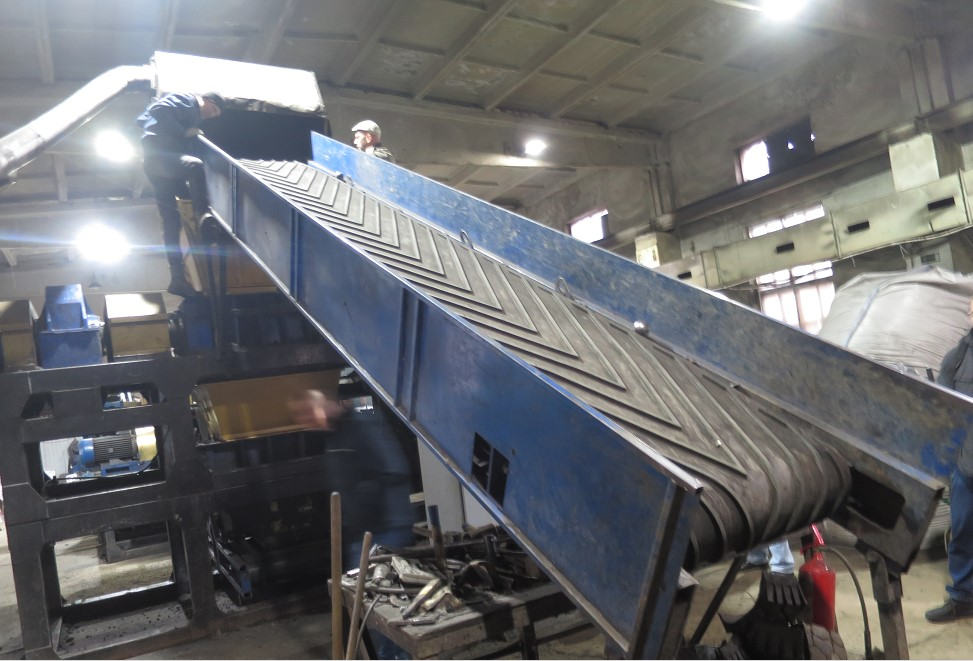
\includegraphics[width=0.85\linewidth]{images/51}
%	\caption{{\footnotesize Левая передняя часть автомобиля \tcm. Стрелки указывают на повреждения передней левой  части автомобиля}} \vspace{10mm} 
%	\label{fig:51}
%\end{figure}
%\vspace{5mm} 
%
%\textbf{Исследование повреждений ходовой части} проводилось с использованием ручного измерительного инструмента и стенда для измерения углов установки колес. 
%\begin{SCfigure}
%	\centering {\footnotesize \caption{ Автодата. Схема рычагов задней подвески }} 
%	\includegraphics[width = 0.4 \textwidth] % 
%	{images/p1} % picture filename 
%\end{SCfigure}
%\begin{SCfigure}
%	\centering {\footnotesize \caption{ Подвеска автомобиля \tcm\, левая повреждённая сторона. Стрелками показаны  деформированные рычаги }} 
%	\includegraphics[width = 0.4 \textwidth] % 
%	{images/50} % picture filename 
%\end{SCfigure}
%\relax
%\begin{figure}[h!]\centering
%	\parbox[t]{0.49\textwidth}
%	{\centering
%		\includegraphics[width=.49\textwidth]{images/p1}
%		\caption{\footnotesize {Автодата. Схема рычагов задней подвески}}
%		\label{fig:p1}}
%	\hfil \hfil
%	\parbox[t]{0.49\textwidth}
%	{\centering
%		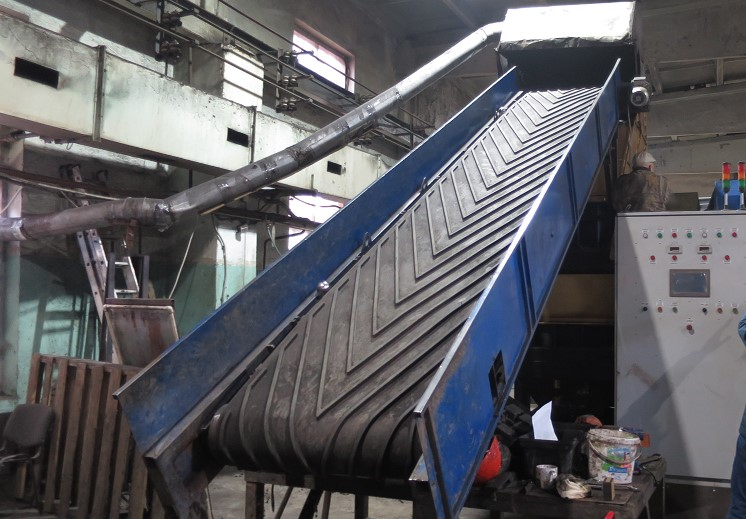
\includegraphics[width=.49\textwidth]{images/50}
%		\caption{\footnotesize { Подвеска автомобиля \tcm\, левая повреждённая сторона. Стрелками показаны  деформированные рычаги }}
%		\label{fig:50}}
%\end{figure}
%\begin{figure}[h!]\centering
%	\parbox[t]{0.49\textwidth}
%	{\centering
%		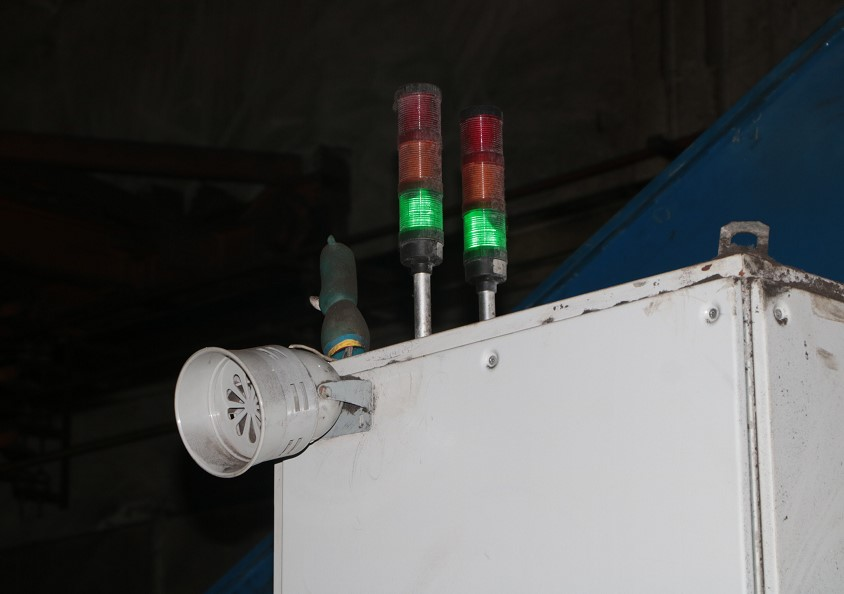
\includegraphics[width=.49\textwidth]{images/47}
%		\caption{\footnotesize {Измерение углов установки колес}}
%		\label{fig:47}}
%	\hfil \hfil
%	\parbox[t]{0.49\textwidth}
%	{\centering
%		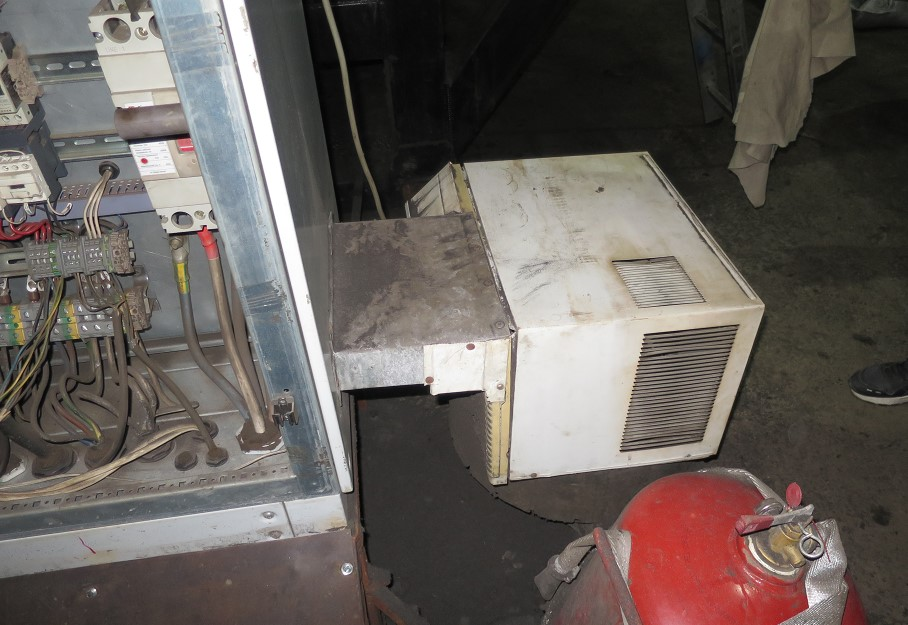
\includegraphics[width=.49\textwidth]{images/48}
%		\caption{\footnotesize { Экран стенда измерения углов установки колес }}
%		\label{fig:48}}
%\end{figure}
%%
%\begin{figure}[h!]
%	\centering
%	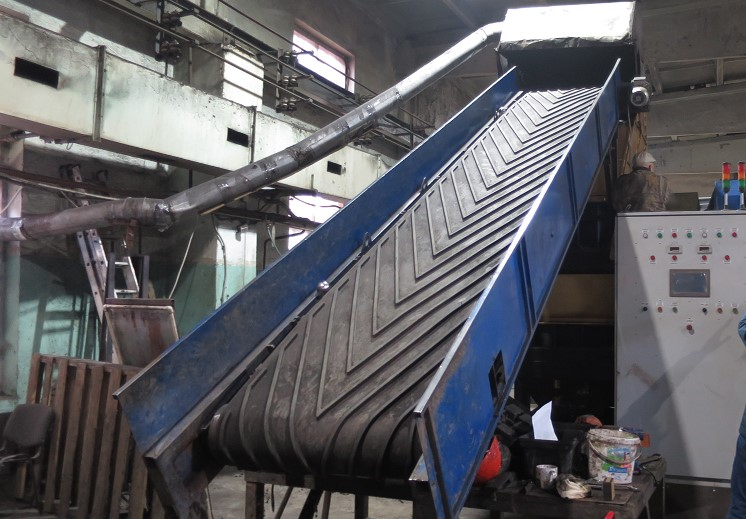
\includegraphics[width=0.9\linewidth]{images/50}
%	\caption[]{{\footnotesize Подвеска автомобиля \tcm\, левая повреждённая сторона. Стрелками показаны  деформированные рычаги}}
%		\label{fig:50}
%\end{figure}
%
%
%
%\begin{figure}[h!]
%	\centering
%	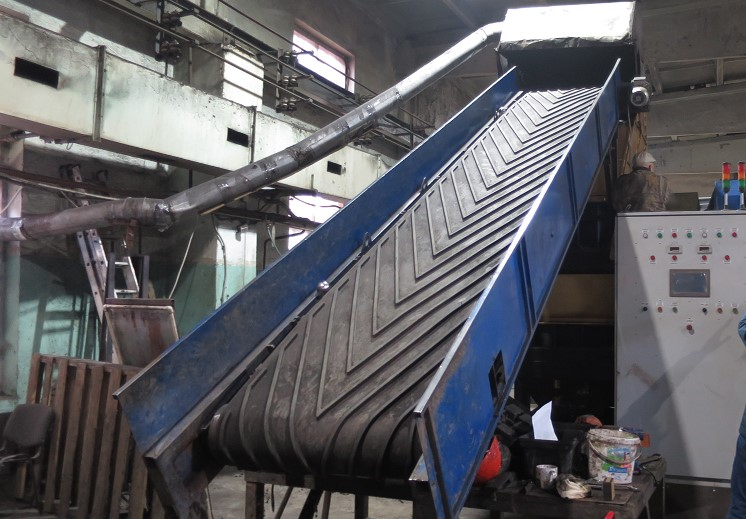
\includegraphics[width=0.85\linewidth]{images/50}
%	\caption[]{{\footnotesize Подвеска автомобиля \tcm\, левая повреждённая сторона. Стрелками показаны  деформированные рычаги}}
%	\label{fig:50}
%\end{figure}
%
%\vspace{10mm}
%   
% \subparagraph*{}\textbf{На предоставленном автомобиле} \tcm\  на момент осмотра раскрыты левая передняя боковая подушка безопасности и левая головная подушка безопасности, Рис. \ref{fig:52}. Система оконных подушек безопасности входит в базовую
% комплектацию модельного ряда W211. Оконные и боковые подушки безопасности срабатывают в том  случае, если центральный электронный блок управления ARMADA регистрирует боковое столкновение. Для определения поперечного  ускорения поступающая от центрального датчика столкновения  информация дополняется информацией от боковых датчиков,
% расположенных в зонах боковых поперечин соответствующих  сторон.
% 
% В результате произведенной проверки электрических цепей системы SRS на наличие повреждений, коррозии, нарушения контактов в   разъемных соединениях  неисправности проводки электрических цепей системы SRS не выявлено. Блок управления системы безопасности в реальном времени нормально реагирует на внешние тестовые воздействия.
% \vspace{3mm}
%\begin{figure}[!h]
%	\centering
%	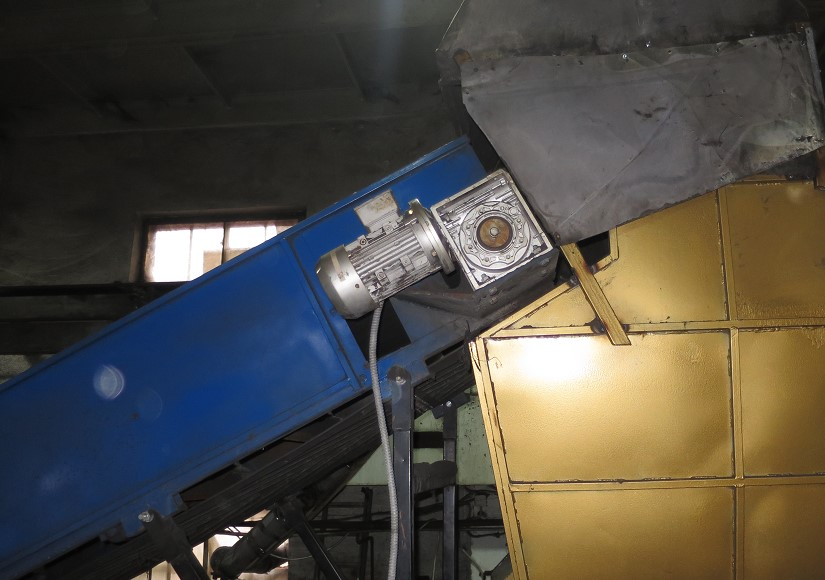
\includegraphics[width=0.85\linewidth]{images/52}
%	\caption{{\footnotesize Автомобиль \tcm с раскрытыми надувными элементами подушек безопасности}}
%	\label{fig:52}
%\end{figure}
%
На автомобиле имеются характерные повреждения 

% \begin{figure}
% 	\centering
% 	\includegraphics[width=0.95\linewidth]{images/screenshot001}
% 	\caption{{\footnotesize Данные блока управления панели комбинации приборов, зафиксированные в процессе исследования автомобиля}}
% 	\label{fig:screenshot001}
% \end{figure}
% \vspace{5mm}
% \begin{figure}[!h]
% 	\centering
% 	\includegraphics[width=0.95\linewidth]{images/d1}
% 	\caption{\footnotesize Снимок экрана компьютера в процессе диагностики системы управления} 	\label{fig:d1}
% \end{figure}
%{\small \begin{enumerate}{\label{en:enum}}
%		\item [] Ошибки системы SRS:
%	\item 92A3 - высокое сопротивление запального контура левой оконной подушки безопасности. Начало ошибки -- ошибка снята: 19 109 126 мотосекунда -- 19 138 962 мотосекунда или 5 308,09 моточасов -- 5 316,37 моточасов);
%	\item 9223 - высокое сопротивление запального контура левой боковой подушки безопасности: 19 109 126 --33 554 430 мотосекунд или 5 308,09 -- 9 320,67 моточасов;
%	\item 92А0 - замыкание (или утечка)на массу в цепи левой оконной подушки безопасности:  19 138 964-- 33 554 430 мотосекунд или  5 316,37 --9 320,67 моточасов.
%\end{enumerate}}
%
%\vspace{-14mm}
%\begin{center}
%	%\renewcommand{\arraystretch}{0.8}ommand{\arraystretch}{0.8}
%%\begin{tabular}{|p{20mm}|p{7cm}|p{25mm}|p{25mm}|}
%%	\hline 
%%	{\footnotesize Код ошибки} & {\footnotesize Описание ошибки} & {\footnotesize Время возникновения, сек} &{\footnotesize  Время окончания, сек} \tabularnewline
%%	\hline 
%%	92A3 & {\small Высокое сопротивление запального контура оконной подушки безопасности} & 19109126 & 19138962 \tabularnewline
%%	\hline 
%%	9233 & {\small Высокое сопротивление запального контура боковой подушки безопасности} & 19109126 & 3355430 \tabularnewline
%%	\hline 
%%	92A0 & {\small Замыкание  в цепи левой оконной подушке безопасности} & 19138964 & 33554430 \tabularnewline
%%	\hline 
%%%	\label{t:pb}
%%\end{tabular}
%%\renewcommand{\arraystretch}{1.2}
%%\begin{tabular}{|p{20mm}|p{7cm}|p{25mm}|p{25mm}|}
%%	\hline 
%%	{\footnotesize Код ошибки} & {\footnotesize Описание ошибки} & {\footnotesize Время возникновения, сек} &{\footnotesize  Время окончания, сек} \tabularnewline
%%	\hline 
%%	92A3 & {\small Высокое сопротивление запального контура оконной подушки безопасности} & 19109126 & 19138962 \tabularnewline
%%	\hline 
%%	9233 & {\small Высокое сопротивление запального контура боковой подушки безопасности} & 19109126 & 3355430 \tabularnewline
%%	\hline 
%%	92A0 & {\small Замыкание  в цепи левой оконной подушке безопасности} & 19138964 & 33554430 \tabularnewline
%%	\hline 
%%%	\label{t:pb}
%%\end{tabular}
%%\renewcommand{\arraystretch}{1.2}}
%\end{center}
%\vspace{3mm}
%Высокое электрическое сопротивление цепи запального контура указывает на активацию газогенератора (пиропатрона). По данным блока SRS, активация газогенераторов обеих подушек безопасности произошла одновременно на 19109126 мотосекунде.  Снятие ошибки 92А3 совпадает (разница 2 секунды) с моментом возникновения ошибки 92А0 (одновременно с образованием замыкания на массу в цепи левой оконной подушки). Т.е. неисправность электрической цепи  системы управления головной подушкой безопасности в виде короткого замыкания или утечки на массу зафиксировано на 8 часов позднее, чем произошла активация системы SRS и, согласно этим данным, не может являться причиной нештатного раскрытия надувного элемента головной подушки.    
%Считанные показания счетчика моточасов работы из блока управления панели приборов -- 53 19,02 ч. или $ \approx 19 148 472 $ мотосекунды, при том, что в блоке SRS содержатся сведения о снятии ошибки на 33 554 430 мотосекунде или 9 320,67 моточасе  работы автомобиля, что есть существенное расхождение во времени работы автомобиля  в различных блоках управления.  Показания одометра на 10.11.2017г. составляли 89 855 км, (акт осмотра ИП Резенькова, л.~д. 30), показания одометра на момент настоящего исследования так же 
%89 855км. Данный факт указывает либо на вмешательство в  блоки управления автомобиля, либо на наличие неисправных блоков управления.  Таким образом, техническое состояние электрических систем исследуемого автомобиля на момент экспертизы не позволяет достоверно определить соответствие срабатывания боковых подушек безопасности заявленному ДТП \dtp.  
%\subsection*{}
%%\vspace{-10mm}
%\vspace{-10mm}\textbf{  Повреждения автомобиля \tca,\, имеющиеся на момент осмотра 02.07.2018:}   
%
%\begin{itemize}
%	
%	\item Капот - остаточная деформация передней части,\, деталь частично восстановлена; 
%	\item Фара левая - заменена;
%	\item Фара правая - разрушен корпус;
%	\item Бампер передний - расколот в левой части, остаточные признаки пластической деформации правой части детали, отслоение ЛКП; 
%	\item Фара правая противотуманная - разбита;
%	\item Облицовка передняя - деформирована;
%	\item Панель рамки радиатора - частично восстановлена геометрия, имеются остаточные деформации;
%	\item Лонжероны передние левые - имеют остаточные деформации передней части деталей;
%	\item Пластина переднего регистрационного знака - деформирована;
%	\item Крыло переднее левое - остаточная деформация, разрывы металла передней угловой части;
%	\item Крыло переднее правое - остаточная деформация, разрывы металла передней угловой части.\\
%	
%\end{itemize}
%\imgh{150mm}{images/38}{Автомобиль \tca\, вид спереди. Расстояние между передними крыльями 1310 мм. Передний верхний угол левого и правого крыла расположены на высоте  720 мм от опорной поверхности.}
%
%\imgh{165mm}{images/mercl}{Автомобиль \tcm\, левая боковина. Расстояние между повреждениями 1310 мм. Расположены на высоте 620...680 мм и 610...670 мм} 
%
%  	Следуя логической последовательности разрешения вопросов настоящей экспертизы,     первоначально необходимо установить механизм взаимодействия автомобилей при заявленных обстоятельствах,  исследовать повреждения транспортных средств,   произвести сопоставление имеющихся повреждений с  механизмом их образования, определить возможность образования повреждений при заявленном событии и только затем определить стоимость восстановительного ремонта повреждений автомобиля \tcm.  Таким образом, эксперт первоначально должен провести  исследование по второму вопросу.
%  
%  \renewcommand\baselinestretch{0.85}\small\normalsize 
% \subsection{\underline{По  вопросу}\, \, \,	\textbf{\small{2. Состоят ли в причинно-следственной связи повреждения транспортного средства Мерседес Бенц регистрационный знак Р781ЕХ93 2003 года выпуска, заявленного истцом с ДТП, имевшем место 31.10.2017г.?}}}  
% \renewcommand\baselinestretch{1.2}\small\normalsize
% 
% %\vspace{-10mm}
%\subparagraph*{}	\parindent=2em  В соответствии с теорией автомобиля и законами механики, взаимодействие  транспортных средств возможно  определёнными зонами	 контактирования на площади перекрытия в вертикальных и горизонтальных плоскостях, исходя из конструктивных особенностей компоновки кузова при геометрическом ориентировании на проезжей части. Соответственно,  образование повреждений на транспортных средствах возможны  в  закономерных направлениях – в продольном направлении: спереди назад или сзади вперёд; в поперечном направлении: слева направо или справа налево;  в комбинированных направлениях при определённых условиях взаимодействия, исходя из особенностей динамики перемещения: спереди назад и сверху вниз, спереди назад и снизу вверх; сзади вперед и сверху вниз; сзади вперед и снизу вверх. Определение механизма столкновения транспортных средств\footnote{С.Я. Евтюков, Я.В. Васильев\,/ Экспертиза ДТП: Методы и технологии/ СПбГАСУ.-Спб., 2012.-310с. ISBN 978-5-9227-0426-7} включает в себя установление траекторий схождения и расхождения транспортных средств; угла между продольными осями транспортных средств в момент их первичного контактного взаимодействия; частей транспортных средств, которыми они впервые вступили в контактное взаимодействие; площади перекрытия контактирующих при ДТП частей транспортных средств; факта состояния покоя или движения транспортных средств в момент первичного контактного взаимодействия; координат места столкновения и расположения транспортных средств относительно неподвижных элементов дороги.% Механизм столкновения устанавливается по следам на транспортных средствах и месте ДТП. Взаимное положение транспортных средств в момент первичного контактного взаимодействия определяется методом натурной реконструкции события ДТП (совмещение и сопоставление пар повреждений на транспортных средствах участвовавших в ДТП) либо при отсутствии такой возможности, по протоколам осмотра транспортных средств и фотографиям их повреждений, приобщенным к материалам дела. По удовлетворению ходатайства \hod транспортные средства на исследование представлены, что позволило эксперту провести натурную реконструкцию взаимодействия транспортных средств, в соответствии заявленному механизму  ДТП. %Установленный механизм взаимодействия автомобилей \tca и \tcm  не противоречит заявленным обстоятельствам ДТП и соответствует условиям перекрестного поперечного столкновения, обусловленного пересечением траекторий движения автомобилей.\,Проведённой в процеcсе исследования натурной реконструкцией столкновения представленных автомобилей   установлено, что правая боковая сторона автомобиля мерседес--бенц Е220  гос.рег.знак Р781ЕХ93 содержит  следы--отображения внешнего строения деталей передней части автомобиля ауди--80 регистрационный знак В393НУ12.
%\vspace{-10mm}
% \subsection*{}
%      \textbf{В результате детального изучения следов на предоставленных ТС  эксперт выделяет следующие контактные пары:}
%\vspace{2mm}
%%\begin{itemize}
%	\item рамка переднего номерного знака \tca и дверь задняя левая \tcm, рис. \ref{ris:images/11}, \ref{ris:images/13}.
%	\item  левая сторона переднего бампера с отверстием  для противотуманной фары  \tca --- дверь передня левая \tcm, рис. \ref{ris:images/46}, \ref{ris:images/32}.
%	\item повреждение левой передней двери \tcm, полученное от контактного взаимодействия с левым передним крылом \tca, рис. \ref{ris:images/35}, \ref{ris:images/36}.
%	\item повреждение левого заднего крыла \tcm, полученное от контактного взаимодействия с правым передним крылом \tca, рис. \ref{ris:images/33}, \ref{ris:images/34}.
%	\item повреждения левой передней и левой задней двери \tcm компрессионного характера - передний бампер ТС, капот, левая и правая фары \tca, рис. \ref{ris:images/37}, \ref{ris:images/38}. 
%	
%\end{itemize}
%\relax
%\begin{figure}[h!]\centering
%	\parbox[t]{0.49\textwidth}
%	{\centering
%		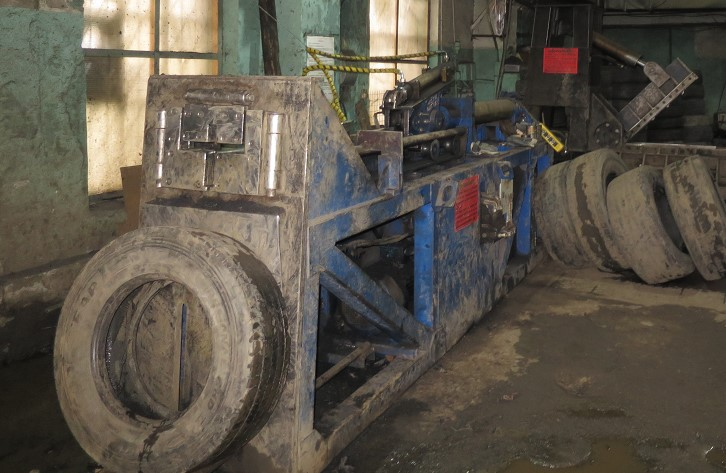
\includegraphics[width=.49\textwidth]{images/1}
%		\caption{\footnotesize {Этапы реконструкции ДТП}}
%		\label{ris:images/1}}
%	\hfil \hfil%раздвигаем боксы по горизонтали 
%	\parbox[t]{0.49\textwidth}
%	{\centering
%		\includegraphics[width=.49\textwidth]{images/39}
%		\caption{\footnotesize {Этапы реконструкции ДТП}}
%		\label{ris:images/39}}
%\end{figure}
%\relax
%\begin{figure}[h!]\centering
%	\parbox[t]{0.49\textwidth}
%	{\centering
%		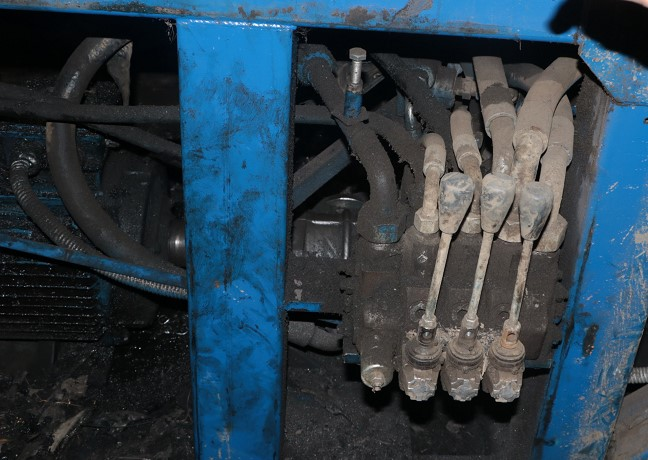
\includegraphics[width=.49\textwidth]{images/11}
%		\caption{\footnotesize {След рамки номерного знака}}
%		\label{ris:images/11}}
%	\hfil \hfil%раздвигаем боксы по горизонтали 
%	\parbox[t]{0.49\textwidth}
%	{\centering
%		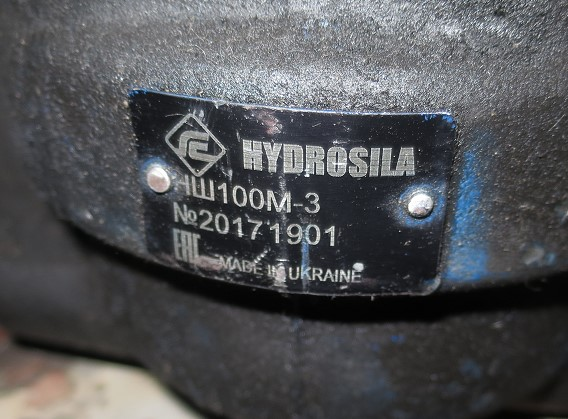
\includegraphics[width=.49\textwidth]{images/13}
%		\caption{\footnotesize {След воздействия правого переднего крыла автомобиля \tca на поверхность крыла заднего левого автомобиля \tcm}}
%		\label{ris:images/13}}
%\end{figure}
%\relax
%\begin{figure}[h!]\centering
%	\parbox[t]{0.49\textwidth}
%	{\centering
%		
\includegraphics[width=.49\textwidth]{images/46}
%		\caption{\footnotesize {левая сторона переднего бампера с отверстием  для противотуманной фары  \tca}}
%		\label{ris:images/46}}
%	\hfil \hfil%раздвигаем боксы по горизонтали 
%	\parbox[t]{0.49\textwidth}
%	{\centering
%		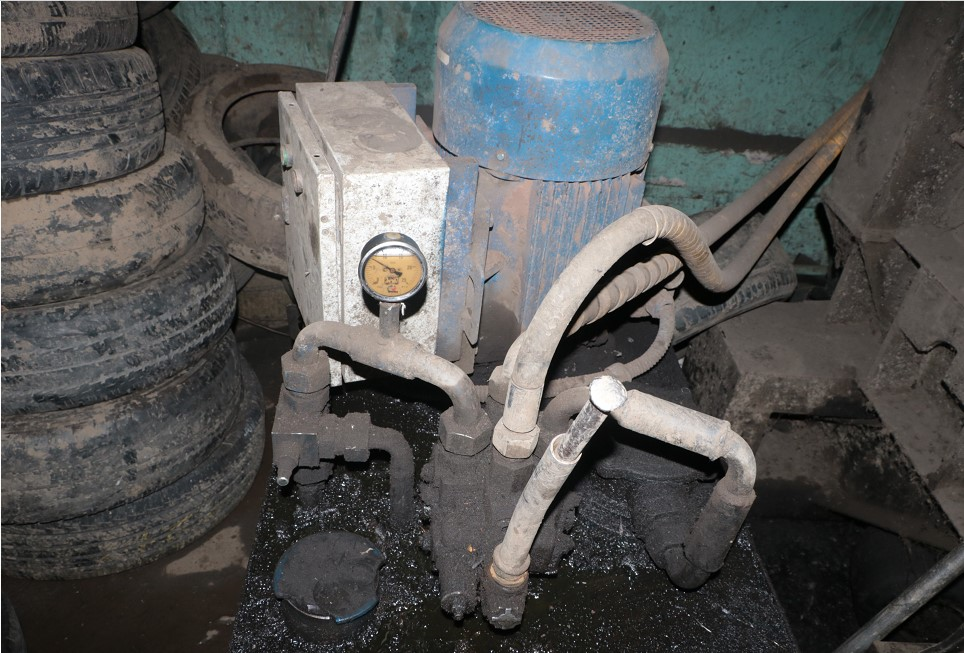
\includegraphics[width=.49\textwidth]{images/32}
%		\caption{\footnotesize {дверь передня левая \tcm}}
%		\label{ris:images/32}}
%\end{figure}
%\relax
%\begin{figure}[h!]\centering
%	\parbox[t]{0.49\textwidth}
%	{\centering
%		\includegraphics[width=.49\textwidth]{images/35}
%		\caption{\footnotesize {Левая передняя дверь автомобиля  \tcm}}
%		\label{ris:images/35}}
%	\hfil \hfil%раздвигаем боксы по горизонтали 
%	\parbox[t]{0.49\textwidth}
%	{\centering
%		\includegraphics[width=.49\textwidth]{images/36}
%		\caption{\footnotesize {Левое переднее крыло автомобиля \tca}}
%		\label{ris:images/36}}
%\end{figure}
%
%\relax
%\begin{figure}[h!]\centering
%	\parbox[t]{0.49\textwidth}
%	{\centering
%		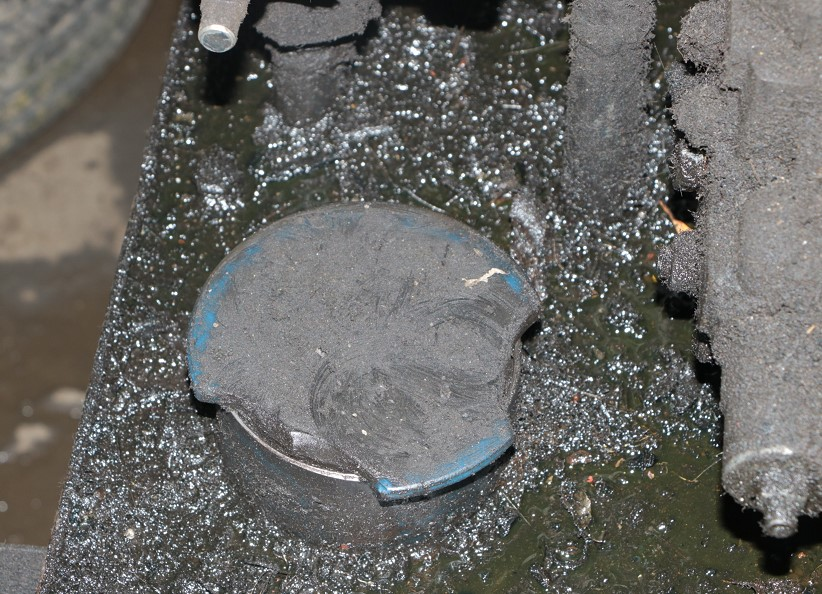
\includegraphics[width=.49\textwidth]{images/33}
%		\caption{\footnotesize {Левое заднее крыло автомобиля \tcm}}
%		\label{ris:images/33}}
%	\hfil \hfil%раздвигаем боксы по горизонтали 
%	\parbox[t]{0.49\textwidth}
%	{\centering
%		\includegraphics[width=.49\textwidth]{images/34}
%		\caption{\footnotesize {Левое переднее крыло автомобиля \tca}}
%		\label{ris:images/34}}
%\end{figure}
%\relax
%\begin{figure}[h!]\centering
%	\parbox[t]{0.49\textwidth}
%	{\centering
%		\includegraphics[width=.49\textwidth]{images/37}
%		\caption{\footnotesize {Левые двери автомобиля \tcm. Следовоспринимающая поверхность}}
%		\label{ris:images/37}}
%	\hfil \hfil%раздвигаем боксы по горизонтали 
%	\parbox[t]{0.49\textwidth}
%	{\centering
%		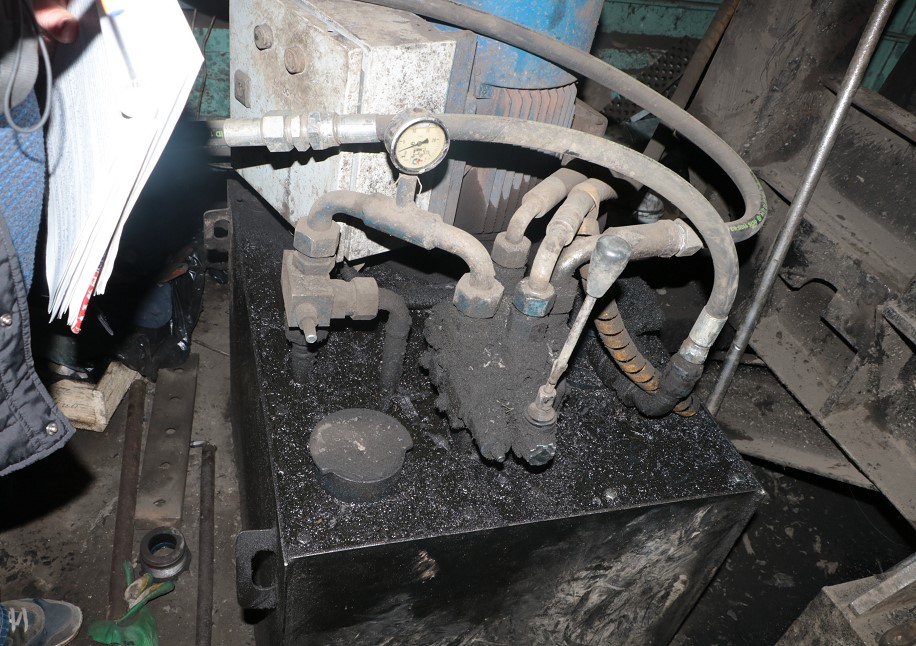
\includegraphics[width=.49\textwidth]{images/23}
%		\caption{\footnotesize {Передний бампер, капот, левая и правая фары \tca. Следообразующая поверхность}}
%		\label{ris:images/23}}
%\end{figure}
%%\rem{Возможно, необходимо перенести в другой раздел}
%\subparagraph*{} Имеющиеся следы комбинированные, статические, направленные перпендикулярно продольной оси автомобиля \tcm с незначительной динамической составляющей  следов внедрения, направленные снизу вверх  и немного слева направо (под углом $ \approx 30^{\circ} $) к вертикальной оси автомобиля.%  рис. \ref{ris:images/1}, \ref{ris:images/39}. \rem{фото характерных следов}
%
%Совокупность индивидуализирующих признаков групп следов и повреждений, имеющихся  на транспортных средствах, совпадающих между собой по уровню расположения, форме и  локализации указывают на   возможность их образования при взаимном контактном взаимодействии по механизму перекрёстного взаимодействия  с центральным ударом.  Различие по высоте ($ \approx 9  \cdots 10 $ см ), в данном случае,  не противоречит  механизму следообразования, так как  закономерность направления деформирующего воздействия со стороны следообразующего объекта на части кузова транспортного средства обусловлены  геометрическими размерами  рассматриваемых объектов, траекторией их перемещения, а также созданием определенных моментов сил,  в том числе вызывающих перераспределение массы по осям, рис.27\ref{ris:images/tormoz}.   Полагаем, что водитель автомобиля \tca, \, перед столкновением с автомобилем \tcm, применил торможение.  Тогда в  момент первичного контакта передняя часть автомобиля  \tca \ была расположена на несколько сантиметров ниже относительно расстояния при нормальных условиях движения или неподвижного состояния, так как согласно законам механики,  в момент торможения происходит перераспределение веса под действием силы
%  \begin{equation}\label{eq:f}
%  \vec{F_t} = \dfrac{\vec{a}*m*H}{L}, \,\,\,\,  \text{где:}
%  \end{equation}
%  \begin{itemize}
%  \item[ ] $\vec{a} $ ---величина замедления;
%  \item[ ] $ L $ --- длина базы автомобиля;  
%  \item[ ] $ H $ --- высота центра тяжести; 
%   \item[ ] $ m $ --- масса автомобиля
%  \end{itemize}
% Действие силы $ \vec{F_t} $   на переднюю ось автомобиля  приводит к дополнительному сжатию пружин передней подвески и, как следствие, уменьшению расстояния от деталей передней части кузова до опорной поверхности. Величина уменьшения расстояния зависит от значения силы $ \vec{F_t} $ и жёсткости  подвески автомобиля.
%В свою очередь,  в начальный момент контакта, положение кузова автомобиля \tcm \, должно было  соответствовать  положению при нормальном  условии движения, далее, под действием силы $ \vec{F_t} = \dfrac{mv^2}{2} $ , где $ m $ -- масса автомобиля \tcm, v -- его скорость, пространственное положение кузова \tcm измениться.
%\imgh{100mm}{images/torm}{Схематичное изображение перераспределения веса при торможении автомобиля }
%\begin{SCfigure}
%\centering \caption{рлрл captioорпоп опрпоп опорпопр опопо  порпорп орор оро опрорп орп ор оорп орп оn text ... } 
%\includegraphics[width = 0.6 \textwidth] % 
%{images/torm} % picture filename 
%\end{SCfigure}
%Анализ характера деформаций и направлений действующих сил, вызвавших повреждения частей деталей правой боковины автомобиля \tcm \, и передней части автомобиля \tca, а именно:
%\begin{itemize}
%	\item[ ] --  обширные площади деформации на ТС в местах, которыми они вошли в контактное взаимодействие с преградой;
%	\item[ ] --  оттиски отдельных участков, деталей одного ТС на поверхности частей другого;
%	\item[ ] --  следы внедрения в виде потёртостей на ТС -- снятия слоя лакокрасочного покрытия, локальных разрывов поверхности;
%	\item[ ] -- трассы (следы скольжения, давления, царапания), возникшие от контакта с другим ТС
%\end{itemize} 
%позволяют заключить, что данные повреждения могли быть образованны в результате  взаимного контактного взаимодействия указанных автомобилей.\\
%Данный механизм следообразования является характерным для \rem{вставить механизм следообразвания}
%Таким образом, сопоставлением характерных групп следов, местом и направлением их нанесения, пространственным совмещением выделенных следовоспринимающих и следообразующих объектов можно сделать общий вывод о наличии пространственно-следового изоморфизма, и соответственно о наличии контактно-следового взаимодействия автомобилей \tca и \tcm.
%
%	Учитывая заявленные обстоятельства ДТП \dtp, исходя из взаимного ориентирования обоих транспортных средств на проезжей части  соответствующими сторонами кузова, а также направления траектории сближения обоих транспортных средств по принципу организации дорожного движения, повреждения левой боковой части автомобиля \tcm могут состоят в причинно-следственной связи с указанным  ДТП. 
%Повреждения деталей передней части автомобиля \тсм, согласно предоставленным административных материалов по данному ДТП, получены в результате наезда автомобиля на дерево, расположенное  на расстоянии 4,6 м от края проезжей части и на удалении $ \approx 10 $ м от места столкновения автомобилей, рис.2. 
%На момент исследования, на автомобиле \тсм имеются остаточные признаки упругой деформации деталей передней левой части автомобиля, по совокупности морфологических признаков не противоречащие заявленному механизму образования. Положение автомобиля \тсм, указанное на схеме ДТП, должно быть обусловлено изменением траектории движения автомобиля после столкновения на угол, составляющий $ \approx 40^\circ $ вправо от направления  движения до столкновения автомобилей. При этом, схема места дорожно-транспортного происшествия не содержит следов потери устойчивости автомобиля после столкновения. Из  анализа механизма взаимодействия автомобилей, эксперт приходит к заключению, что положение автомобиля \тсм, указанное  на схеме ДТП не является результатом изменения траектории его  движения  вследствие удара, а вероятно, связано с управляющими действиями водителя, его ответной реакцией на столкновение.
%Следовательно, повреждения деталей передней части автомобиля \tcm могут находится в причинно-следственной связи с указанным  ДТП.% так как  характер повреждений  не противоречит заявленным обстоятельствам. 
%\subparagraph*{}Таким образом, по совокупности признаков, эксперт приходит к выводу о том, что  повреждения транспортного средства Мерседес Бенц регистрационный знак Р781ЕХ93 2003 года выпуска  состоят  в причинно-следственной связи с  ДТП, имевшем место 31.10.2017г.
%{\begin{enumerate}
%		
%	\item Наличие чётких отпечатков частей одного ТС на другом в местах их первичного контакта при отсутствии трасс местах образования отпечатков или при наличии трасс, возникших после образования отпечатков \rem{еще ремарка по ударв неподвижное тс}
%	\item  Совпадение направления первоначальных трасс и деформаций на ТС, по которому был нанесен удар при перекрёстном столкновении,  направлением движения другого ТС
%	\item Расположение трасс тангенциальной направленности на боковой поверхности колес
%	\item Разворот ТС в направлении момента, который мог возникнуть при столкновении только в случае движения тс, по которому был нанесён удар \\
%	
%	 
%\end{enumerate}}
%Необходимо отметить \rem{опять про изоморфизм}, что данный вид трасологических исследований (установление пространственно-следового изоморфизма, а
%именно установление факта контактно-следового взаимодействия,
%сопоставление обстоятельств ДТП, заявленных страхователем с механизмом нанесения повреждений и т.д.) в настоящее время становится все более и более востребованным и актуальным, т.к. в современных условиях складывается ситуация, когда мошенничество на
%транспорте, с целью получения страхового возмещения, приобретает объёмы снежного кома.
%%%%%%%%%%%%%%%%%%%%%%%%%%%%%%%%%%%%%%%%%%%%%%%%%%%%%%%%%%%%%%%%%%%%%%%%%%%%%%%%%%%%%%%%%%%%%%%%%%%%%%%%%%%%%%%%%%%%%%%%%%%%%
\renewcommand\baselinestretch{0.86}\small\normalsize 
\subsection{\underline{По  вопросу}\, \, \,	\textbf{\small{"Определить стоимость восстановительного ремонта с учетом износа стоимости запасных частей"?}}}
\renewcommand\baselinestretch{1.2}\small\normalsize
Колесное транспортное средство сроком эксплуатации более 7 лет относится к категории транспортных средств с граничным сроком эксплуатации [1], для которой возможно применение ремонтных операций при условии экономической целесообразности и  технической возможности.  

В соответствии с принятой экспертной методикой [1], стоимость восстановительного ремонта АМТС  $ C_p $ определяется по формуле:
%
\begin{equation}\label{eq:r}
C_\text{вp} =C_p + C_\text{м} + C_\text{зч}\cdot\left( 1-\frac{\text{И}}{100}\right)  \,\,\,\, \text{где:}
\end{equation}
%
%
\begin{itemize}
	%	
	\item[ ]$C_\text {р} $ --  стоимость ремонтных работ по восстановлению КТС, руб.;
	\item[ ]$ C_\text{м} $ --  стоимость необходимых ремонтных материалов, руб.;
	\item[ ]$ C_\text{зч} $ --  стоимость новых запасных частей, руб;
	\item[ ] $ \text{И} $ -- коэффициент износа составной части, подлежащей замене, \%.
\end{itemize}
%
%
Коэффициент износа составных частей (И) КТС (кроме автобусов и грузовых автомобилей) при определении стоимости восстановительного ремонта расчитывается по формуле:

\begin{equation}\label{eqsnos}
\text{И} =\text{И1}\cdot\text{П}+\text{И2}\cdot \text{Д}, \%  \,\,\,\, \text{где:}
\end{equation}

\begin{itemize}
	\item [] $ \text{И1} $ --усредненный показатель износа на 1000 км пробега, \%; 
	\item [] $ \text{П} $ -- общий пробег (фактический или расчетный) за срок эксплуатации КТС, тыс.км;
	\item [] $ \text{И2} $ -- усредненный показатель старения за 1 год эксплуатации, \%;
	\item [] $ \text{Д} $ -- срок эксплуатации КТС (от даты изготовления КТС до момента, на который определяется износ), лет. 
\end{itemize}

Для исследуемого автомобиля \тс, согласно справочным таблицам [1]:
\begin{equation}\label{eqsnosr}
\text{И} =\text{И1}\cdot\text{П}+\text{И2}\cdot \text{Д} = 0.23\cdot 214  + 0.85\cdot 9 = 49 \, \%
\end{equation}
%%%%%%%%%%%%%%%%%%%%%%%%%%%%%%%%%%%%%%%%%%%%%%%%%%%%%%%%%%%%%%%%%%%%%%%%%%%%%%%%%%%%%%%%%%%%%%%%%%%%%%%%%%%%%%%%
%Стоимость восстановительных работ $ C_{\text{вр}} $ определяется на основании норм трудоёмкостей $ T_i $, \,предусмотренных заводом-изготовителем, и стоимостных параметров $ C_{i\text{нч}} $ (стоимости нормо-часа) работ по техническому обслуживанию и ремонту АМТС. 
%\begin{equation}\label{eq:cr}
%C_{\text{вр}}  =\sum{C_{ip}}= \sum\left({T_{ij}}\cdot {C_{i\text{нч}}}\right) + \sum{C_{ip^{\text{\,\,\,руб}}}} , \,\,\,\text{где:} 
%\end{equation}
%\vspace{2mm}
%\begin{itemize}
%	\item[ ]$ C_{ip} $ -- стоимость работ i-го вида: $C_\text {зам} $, $ C_\text{восст} $, $ C_\text{рег} $, $C_\text{контр} $, $ C_\text{антикор} $, $ C_\text{зч} $, $ C_\text{ом} $,$ C_\text{соп} $, $ C_\text{вм} $, руб;
%	\item[ ]$ T_{ij} $ -- трудоёмкость j-й операции(комплекса) по i-му виду работ, руб;
%%	\item[ ]$ C_{i\text{нч}} $ -- стоимость нормо-часа по i-му виду работ, руб;
%	\item[ ]$ C_{ip^\text{\,\,руб}} $ -- стоимость работ $ C_{ip} $, принятая непосредственно в денежном выражении, руб.
%\end{itemize}
%
%\vspace{5mm}
%При определении стоимости восстановительного ремонта АМТС с учётом износа под износом следует понимать количественную меру физического старения АМТС и его элементов, достигнутого в результате эксплуатации, т.е. эксплуатационный износ.\\
%%
%Расчёт износа производится в  соответствии с Положением Банка России от «19» сентября 2014 года № 432-П «О единой методике определения размера расходов на восстановительный ремонт в отношении повреждённого транспортного средства» [3].
%Износ комплектующих изделий (деталей, узлов, агрегатов) рассчитывается по следующей формуле:
%
%\begin{equation}\label{eq:I}
%\text{И}_{\text{ки}} 
%= 100\cdot\left( 1-e^ {-\left( \Delta_{T} \cdot T_{\text{КИ}} + \Delta_{L} \cdot L_{\text{КИ}} \right)}\right), \,\,\,\,\text{где:}   
%\end{equation}
%
%\begin{itemize}
%	\item[ ]$ \text{И}_{\text{ки}} $ -- износ комплектующего изделия (детали, узла, агрегата) (процентов); 
%	\item[ ]$ e $ -- основание натуральных логарифмов (e =  2,72);;
%	\item[ ]$ \Delta_{T}$ --  срок эксплуатации комплектующего изделия (детали, узла, агрегата) (лет);
%	\item[ ]$ T_{\text{КИ}} $ -- стоимость работ $ C_{ip} $, принятая непосредственно в денежном выражении, руб
%	\item[ ]$ \Delta_{L} $ --коэффициент, учитывающий влияние на износ комплектующего (детали, узла, агрегата) величины пробега транспортного средства с этим комплектующим изделием;
%	\item[ ]$ L_{\text{КИ}} $ --пробег транспортного средства на дату дорожно-транспортного происшествия (тысяч километров).  
%		\end{itemize}
%\vspace{5mm}
%Значения коэффициентов $ \Delta_{T}$  и $ \Delta_{L} $  для различных категорий и марок транспортных средств приведены в п.5. исп. лит~[3]. При этом, на комплектующие изделия (детали, узлы, агрегаты), которые находятся в заведомо худшем состоянии, чем общее состояние транспортного средства в целом, и его основные части, вследствие влияния факторов, не учтённых при расчете износа (например, проведение ремонта с нарушением технологии, не устранение значительных повреждений лакокрасочного покрытия), может быть начислен дополнительный индивидуальный износ. 
%Износ шины транспортного средства рассчитывается по следующей формуле:
%\begin{equation}\label{eq:sh}
%\text{И}_{\text{ш}} = \frac{\text{Н}_{\text{н}}-\text{Н}_{\text{ф}}}{\text{Н}_{\text{н}}-\text{Н}_{\text{доп}}} \cdot{100}\%  \,\,\,\,\text{где:} 
%\end{equation}
%
%\begin{itemize}
%	\item[ ] $ \text{И}_{\text{ш}} $ -- износ шины, \%;
%	\item[ ] $ \text{Н}_{\text{н}} $ -- высота рисунка протектора новой шины, мм;
%	\item[ ] $\text{Н}_{\text{ф}} $ -- фактическая высота рисунка протектора шины, мм;
%	\item[ ] $ \text{Н}_{\text{доп}} $ --минимально допустимая высота рисунка протектора шины в соответствии с требованиями законодательства Российской Федерации, мм.
%\end{itemize}
%
%\renewcommand\baselinestretch{1}\small\normalsize
%
%Износ шины дополнительно увеличивается для шин с возрастом от 3 до 5 лет - на 15 процентов, свыше 5 лет - на 25 процентов.
%
В результате исследования   экспертом установлено, что для устранения повреждений \тс \, необходимо  выполнить следующие  работы:
\begin{center}
	\begin{tabulary}{\textwidth}{LCL}
		\hline 
		\textbf{Наименование детали}      &   & \textbf{Ремонтное воздействие}\\
		\hline    
		Турбина левая     &   &    Заменить\\
		Блок ДВС    &   &    Отремонтировать гильзованием, заменой колец и прокладок \\
		Головка блока цилиндров & & Восстановить седла клапанов пятого цилиндра \\
		Впускной тракт & &    Разобрать, прочистить\\
		Интеркулер   & &     прочистить\\
		
		
	\end{tabulary}  
\end{center}
\renewcommand\baselinestretch{1.2}\small\normalsize
%
\textbf{Произвести  необходимые для выполнения  ремонта разборочно-сборочные, подготовительные и вспомогательные работы в соответствии с требованиями завода–изготовителя транспортного средства.}\\
%
Расчет стоимости восстановительных расходов выполнен в программе \auda. \\ Ниже представлены результаты расчета, полная калькуляция стоимости ремонта включена в раздел Приложение.
%%\smallskip
\begin{figure}[H]
	\centering
	\includegraphics[width=0.8\linewidth]{images/Screenshot_2}
	%%	\caption{}
	%%	\label{fig:screenshot001}
\end{figure}
%\begin{figure}[H]
%	\centering
%	\includegraphics[width=0.9\linewidth]{images/screenshot002}
%%%	\caption{}
%	\label{aud}
%\end{figure}
\medskip
Стоимость коммерческого нормо-часа работ применена  с учетом условий регионального рынка услуг и сложившихся средних расценок по видам работ, типу ТС, а также по маркам и моделям ТС  и   составляет  1300 р/ч для данного транспортного средства. \\
Трудоёмкость работ по разборке/сборке/замене  соответствует трудоемкости работ, рекомендованной заводом изготовителем ТС. 
Расчет стоимости ремонта, согласно положениям [1] производится с учетом  применения оригинальных запасных частей, которые поставляются изготовителем КТС авторизованным ремонтным организациям. Техническое состояние запасных частей учитывается коэффициентом износа, что в совокупности с установкой оригинальных запасных частей в максимальной степени отвечает понятию «восстановительный ремонт», то есть восстановления состояния КТС, при котором используются установленные изготовителем составные части, но с использованным частично ресурсом. 

%
В результате проведенных расчетов (см. Приложение, калькуляция № 22-2019) определена стоимость восстановительного ремонта транспортного средства  \тс, которая составляет 441 295 (Четыреста сорок одна тысяча двести девяносто пять) рублей без учета износа,
стоимость восстановительных расходов, с учетом уменьшения стоимости запасных частей вследствие их износа,  составляет 281 990 (двести восемьдесят одна тысяча девятьсот девяносто) рублей.

\section{Результаты исследования}

\section{Выводы}

\subparagraph*{}
%	

{\small 
	\begin{longtable}{|p{4mm}|p{10mm}|p{16mm}|p{5cm}|p{6cm}|}
		\caption[]{\footnotesize {\textbf{$\cdots$}}} \label{tab:5}\\
		\hline
		%\rowcolor[HTML]{C0C0C0} 
		% Заголовки столбцов
		\text{n/n} &\textbf{Дата} &\textbf{Пробег,\~км}& \textbf{Причина обращения }& \textbf{Выполнено } \\ \hline \endhead % повторение заголовка 
		% Строки
		\Rownum &  & n& Панель задка  & Замена, окраска \\ \hline
		%\rowcolor[HTML]{EFEFEF} 
		\Rownum & &n & Боковина задняя левая   & Замена, окраска \\ \hline
		%%% ..............& 
		
\end{longtable}}\setcounter{rownum}{0}


\begin{enumerate}
	\item \textbf{"Причина поломки или неисправности ДВС на автомобиле Toyota Land Cruizer 200, 2008 года выпуска VIN: JTMHV05J004031859, после проведения ремонта ответчиком при изложенных в исковом заявлении обстоятельствах является попадание постороннего предмета, а именно болта крышки клапанов в левый впускной тракт, что привело к разрушению колеса турбины и повреждению рабочих поверхностей пятого цилиндра ДВС}
	
	\vspace{5mm}
	
	\item \textbf{ Стоимость восстановительного ремонта с учетом износа стоимости запасных частей составляет 281 990 (двести восемьдесят одна тысяча девятьсот девяносто) рублей}
\end{enumerate}
\vspace{15mm}
\relax
Приложение к заключению:\\
\textit{
	Расшифровка комплектации ТС по VIN \\
	Листинг калькуляции стоимости восстановительных расходов\\
}

\vspace{20mm}

